\subsection{Build and Deployment Guide}
\label{subsec:build_deploy}
The build and deployment of the alamSYS docker compose are 
covered in this section. The discussion is divided into two sections. 
The first section discusses how to build and run the alamSYS docker compose. 
The second section discusses the current implementation's deployment using a 
low-cost tunneling service.

\subsubsection{Building and Running Docker Compose of alamSYS}
\label{subsubsec:docker_build}
% Introduction
The alamSYS is deployed using docker compose containers, 
which is a docker tool that allows multiple containers to run concurrently. 
The docker compose file, on the other hand, is specific to the alamSYS and 
runs three containers: alamPREPROCESSOR, alamAPI, and alamDB.


% Initialization of .env files (db.env and preprocessor.env)
Assuming the server device already has docker installed and a copy of the alamSYS 
source code, which can be accessed via the link in Appendix A, the following '.env'
files should be created and added to the alamSYS root folder.
\\

The first '.env' file is the 'db.env' file, which contains the alamDB's 
environment variables. Wherein, the file contains the following details 
as indicated in the code snippet below.
\hfill \\
\begin{python}
    # MongoDB
    MONGO_INITDB_DATABASE="alamAPI_DB"
    MONGO_HOST="mongo_db"
    MONGO_PORT=27017

    # Timezone
    TZ="Asia/Hong_Kong"
\end{python}

And the other '.env' file is the 'preprocessor.env', which contains the 
alamPREPROCESSOR's environment variables. Wherein, the file contains the following 
details as indicated in the code snippet below. Note that the EOD\_API\_KEY
indicated should be changed to the actual API KEY provided in the account of 
the user and should not be shared to anyone or publicly. Moreover,
other than the API KEY, there is nothing to be changed.
\hfill \\
\begin{python}
    # Change API KEY to actual API KEY value
    EOD_API_KEY=000000000000

    # MongoDB
    MONGO_INITDB_DATABASE="alamAPI_DB"
    MONGO_HOST="mongo_db"
    MONGO_PORT=27017

    # Timezone
    TZ="Asia/Hong_Kong"

    # ml_processor
    MODEL_PATH="model"
\end{python}

At the end the folder structure of the alamSYS, should look like
the one indicated in Figure \ref{fig:alamSYS_foldStruct}.
\begin{figure}[ht]
    \centering
    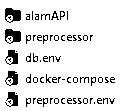
\includegraphics[height=0.15\textheight]{./assets/Chapter_4/Documentation/alamSYS_folder.png}
    \caption{alamSYS Required Folder Structure}
    \label{fig:alamSYS_foldStruct}
\end{figure}
\FloatBarrier

% Docker-compose file and docker file screenshots
After creating and adding the necessary '.env' files to the alamSYS root 
folder. Using the following command, we can now build and run the 
docker compose command from the terminal:
\hfill \\
\begin{python}
    docker-compose build && docker-compose up
\end{python}

The aforementioned command creates the alamSYS containers and then runs them 
all. Furthermore, in subsequent runs, simply run the second part of the 
command 'docker-compose up' to initialize the alamSYS containers. 
Only build the containers on the first initialization or if the alamSYS 
source code has changed.

\subsubsection{Deployment using Network Tunnelling Services}
\label{subsubsec:deploymeny_tunnel}
% Introduction
In order to minimize the cost of alamSYS deployment, the developer 
decided to use the LocalXpose service, which is a network tunneling service. 
It is a reverse proxy that allows you to expose your localhost services 
to the internet and can be found at https://localxpose.io/docs/
\\

% Instructions for running the tunnelling service with the Windows CLI
LocalXpose's official documentation contains device-specific 
instructions. Whereas, the deployment instructions in this section are based 
on the Windows 11 operating system.
\\

To begin, we must create a reserved domain in the LocalXpose Dashboard, 
which can be accessed via this link: https://localxpose.io/dashboard/domain.  
In the case of alamSYS, the reserved domain was set to the Asia Pacific (AP) 
region in order to maintain relatively strong data transfers. Following that, 
the user must download the binary program for their device's operating system; 
in the author's case, he downloaded the Windows 64-bit binary file.
\\

The user should launch the command prompt (cmd) from the directory containing 
the downloaded file. It should be noted that, as of the writing of this paper, 
the binary file only works with cmd, and using powershell or windows terminal 
causes errors. To run the binary application loclx, 
enter the following command into cmd:
\hfill \\
\begin{python}
    loclx.exe account login
\end{python}

The LocalXPose application would then prompt the user for an access token, 
which can be obtained at https://localxpose.io/dashboard/access. 
Following that, the user should enter the following command:
\hfill \\
\begin{python}
    loclx tunnel http --reserved-domain [reserved.domain] --to 8000
\end{python}

The last command launches the localx tunnel command in http mode with a 
reserved domain. And the value 8000 at the end indicates that the reserved 
domain will expose port 8000. This corresponds to the alamAPI's network port, 
making the alamAPI accessible via any network with an internet connection. 
It should also be noted that the user should replace '[reserved.domain]' 
with the actual reserved domain they created in the LocalXpose Dashboard.
Finally, the application will now show the status of the connection.
